% Provenance (never printed): see sources/outline_sources.md (Year 2: the solar nebula
% and the condensation sequence; planetesimals and embryos; chondrites, achondrites and
% irons; the age of the Solar System; differentiation of planets). Curves from
% figdata/bachelor-2/nebula.py, condensation.py, al26.py, meteorites.py; exercise and
% problem values in the Book 4 scratch calculator calc/ch02.py.
\chapter{De vorming van planeten en meteorieten}\label{ch:b2:planet-formation-meteorites}

Elk jaar komen zo'n vijftienduizend ton stof uit de ruimte de dampkring van de aarde
binnen; het meeste ervan verbrandt of zakt neer als microscopische bolletjes, en heel
af en toe valt een steen ter grootte van een vuist neer met een vuurbol en een knal.
De meeste van deze stenen zijn stukken van planetoïden, en veel ervan zijn nauwelijks veranderd
sinds hun vorming. Zaag er een open en polijst hem, en hij toont millimetergrote
bolletjes van ooit gesmolten gesteente, witte onregelmatige korrels van calcium- en
aluminiumhoudende mineralen, schilfers metaal, alles bijeengehouden door een donker, fijnkorrelig cement. De witte
korrels zijn de oudste vaste stoffen van het zonnestelsel: loodisotopen dateren ze op
4567 miljoen jaar. Een tweede klok, het verval van een radioactieve isotoop van
aluminium die al lang verdwenen is, dateert de andere bestanddelen ten opzichte van
deze korrels tot op een fractie van een miljoen jaar. Dit hoofdstuk volgt de schijf van
het vorige hoofdstuk terwijl ze in planeten overgaat: welke vaste stoffen uit het afkoelende gas
condenseren, en waar; hoe stof uitgroeit tot lichamen van kilometers groot en daarna
tot planeten; wat \omterm{def:b2:planet-formation-meteorites:fall-find}{meteorieten} zijn, en hoe ze deze gebeurtenissen dateren; en waarom
sommige van de eerste lichamen smolten en een ijzeren kern kregen, terwijl andere bleven zoals ze
gevormd waren.
% ledger: rojas21:flux, lugaro:cai, gail:meteorites

\begin{recall}
Jonge sterren zijn omgeven door \omterm{def:b2:ism-star-formation:disc}{protoplanetaire schijven}, die binnen enkele
miljoenen jaren verdwijnen; een korrel in sterlicht op afstand $r$ van een ster met
lichtkracht $L$ komt op $T = \bigl(L/(16\pi\sigma r^2)\bigr)^{1/4}$
(\cref{ch:b2:ism-star-formation}). Planetoïden zijn de kleine rotsachtige of metalen
lichamen van het zonnestelsel, waarvan de meeste tussen Mars en Jupiter draaien
(Boek~3). Een radioactieve kern vervalt met de kans $\lambda$ per
tijdseenheid: $N = N_0 e^{-\lambda t}$; de halveringstijd is $\ln 2/\lambda$, en de gemiddelde
levensduur $\tau = 1/\lambda$ (natuurkunde). In een gesloten systeem liggen cogenetische monsters met
verschillende verhoudingen van moeder- tot dochterisotoop op een rechte lijn, de isochroon, waarvan de
helling de ouderdom geeft en het snijpunt met de as de beginverhouding (Boek~3).
Een massa $m$ met soortelijke warmte $c$ over $\Delta T$ opwarmen vergt de energie
$mc\,\Delta T$ (natuurkunde).
\end{recall}

\section{De zonnenevel}

\begin{definition}[Zonnenevel]\label{def:b2:planet-formation-meteorites:nebula}
De \emph{zonnenevel}\index{zonnenevel} is de \omterm{def:b2:ism-star-formation:disc}{protoplanetaire schijf} van gas
en stof die de jonge Zon omringde en waaruit de planeten, hun
manen, de planetoïden en de kometen ontstonden.
\end{definition}

Hoeveel materie bevatte hij? Een ondergrens komt van de planeten zelf.
Voeg aan elke planeet genoeg waterstof en helium toe om haar de samenstelling van de
Zon te geven, spreid het resultaat uit over een ring rond haar baan, en de
oppervlaktedichtheid, de massa per oppervlakte-eenheid van de schijf, neemt af met de afstand tot
de Zon. Deze reconstructie is de \emph{zonnenevel met minimale
massa}\index{zonnenevel met minimale massa}. In een veelgebruikte versie is de
oppervlaktedichtheid van het gas
\[
  \Sigma_g = \qty{2200}{g.cm^{-2}}\left(\frac{r}{\qty{1}{au}}\right)^{-3/2},
\]
en die van de vaste stoffen $\Sigma_p = \qty{33}{g.cm^{-2}}\,Z_{\mathrm{rel}}\,
(r/\qty{1}{au})^{-3/2}$, waarin $Z_{\mathrm{rel}}$ de fractie is van de
condenseerbare materie die werkelijk vast is: $0.33$ waar alleen gesteente en metaal zijn
gecondenseerd, ongeveer $0.78$ waar waterijs zich erbij heeft gevoegd, $1$ voorbij de plaats
waar methaan bevriest. De getallen zijn onzeker: het gehalte aan zware elementen van
Jupiter is slechts op een factor vier na bekend, en de planeten hoeven niet
ontstaan te zijn waar ze nu draaien.
% ledger: cy10:mmsn

\begin{proposition}[Massa van een schijf]\label{prop:b2:planet-formation-meteorites:disc-mass}
Een schijf met oppervlaktedichtheid $\Sigma(r) = \Sigma_1 (r/r_1)^{-3/2}$ bevat binnen
de straal $R$ de massa
\[
  M(R) = 4\pi\Sigma_1 r_1^2 \left(\frac{R}{r_1}\right)^{1/2}.
\]
Het grootste deel van de massa ligt ver naar buiten: een verdubbeling van de straal voegt \qty{41}{\percent} toe aan
de massa.
\end{proposition}

\begin{proof}
Een ring met straal $r$ en breedte $\mathrm dr$ heeft de oppervlakte $2\pi r\,\mathrm dr$, dus
\[
  M(R) = \int_0^R 2\pi r\,\Sigma_1 \left(\frac{r}{r_1}\right)^{-3/2}\mathrm dr
       = 2\pi\Sigma_1 r_1^{3/2}\int_0^R r^{-1/2}\,\mathrm dr
       = 4\pi\Sigma_1 r_1^{3/2} R^{1/2},
\]
wat de formule is; de integraal convergeert in $r = 0$. Een verdubbeling van $R$
vermenigvuldigt $M$ met $\sqrt 2 = 1.41$.
\end{proof}

Met $\Sigma_1 = \qty{2.2e4}{kg.m^{-2}}$ bij $r_1 = \qty{1}{au}$ bevat de nevel met minimale
massa $0.03$ zonsmassa binnen \qty{100}{au} (\cref{exo:b2:planet-formation-meteorites:5}). De schijven
die rond sterren van een miljoen jaar oud worden waargenomen, gewogen met de millimetergloed van
hun stof, bevatten \numrange{0.001}{0.1} zonsmassa: de nevel met minimale massa
valt daar ruim binnen.
% ledger: cy10:mmsn

Bijna al deze massa is gas dat nooit zal condenseren. De Zon werd geboren
met een massafractie waterstof $X_0 = 0.711$, helium $Y_0 = 0.274$ en
alle zwaardere elementen samen slechts $Z_0 = 0.0149$. Een gas met deze
samenstelling afkoelen tot alles wat kan bevriezen bevroren is, zet slechts
\qty{1.5}{\percent} van zijn massa om in vaste stoffen: \qty{0.49}{\percent} gesteente en
metaal, en \qty{1.0}{\percent} ijs van water, methaan en ammoniak, waarvan waterijs
alleen \qty{0.57}{\percent} is. Alle rotsachtige planeten, en de kernen van de
reuzen, zijn uit deze kleine fractie opgebouwd.
% ledger: lodders:protosolar, lodders:condensates

De temperatuur van de schijf bepaalt wat waar vast is. Een schijf die alleen door
haar ster wordt verwarmd, een \emph{passieve} schijf, is warm aan haar oppervlak, waar de korrels
de ster rechtstreeks zien (de propositie van \cref{ch:b2:ism-star-formation}), en
veel kouder in haar middenvlak, dat alleen het infrarood ontvangt dat door
die oppervlaktekorrels opnieuw wordt uitgezonden. Voor een jonge ster van één zonsmassa geeft een model van zo'n schijf
de temperatuur in het middenvlak
\[
  T = \qty{120}{K}\left(\frac{r}{\qty{1}{au}}\right)^{-3/7}.
\]
Accretie van gas door de schijf, die gravitatie-energie vrijmaakt, maakt
het middenvlak heter, vooral in het begin en dicht bij de ster (figuur hieronder).
% ledger: cy10:passive

\begin{omfigure}
\begin{tikzpicture}
\begin{axis}[omrecord, width=0.82\linewidth, height=6.2cm, xmode=log, ymode=log,
  xmin=0.1, xmax=100, ymin=10, ymax=1000,
  xlabel={afstand tot de ster $r$ (au)}, ylabel={temperatuur (K)},
  tick label style={font=\scriptsize}, label style={font=\small},
  legend pos=north east, legend style={font=\scriptsize, draw=black!30}]
\addplot[thick, red!70!black] table[x=r_au, y=T_grain] {figdata/out/bachelor-2-nebula-temp.dat};
\addlegendentry{korrels in direct sterlicht}
\addplot[thick, blue!70!black] table[x=r_au, y=T_mid] {figdata/out/bachelor-2-nebula-temp.dat};
\addlegendentry{middenvlak van een passieve schijf}
\addplot[black!50, densely dashed, domain=0.1:100, samples=2] {182};
\addplot[black!50, densely dashed, domain=0.1:100, samples=2] {41};
\node[font=\scriptsize, anchor=south east] at (axis cs:95,182) {waterijs, \qty{182}{K}};
\node[font=\scriptsize, anchor=north west] at (axis cs:0.46,41) {methaanijs, \qty{41}{K}};
\draw[blue!70!black, -latex] (axis cs:0.38,25) -- (axis cs:0.38,175);
\node[font=\scriptsize, blue!70!black, anchor=north] at (axis cs:0.38,25) {\qty{0.4}{au}};
\draw[red!70!black, -latex] (axis cs:2.34,25) -- (axis cs:2.34,175);
\node[font=\scriptsize, red!70!black, anchor=north] at (axis cs:2.34,25) {\qty{2.3}{au}};
\end{axis}
\end{tikzpicture}

\par\smallskip{\small Twee temperaturen van een schijf rond een ster met één zonslichtkracht.
Rood: een zwarte korrel in direct sterlicht (\cref{ch:b2:ism-star-formation}). Blauw: het
middenvlak van een passieve schijf rond een jonge ster van één zonsmassa, afgeschermd van direct
licht. Waterijs is stabiel onder \qty{182}{K}: de pijlen geven aan waar elke kromme
die lijn snijdt. De werkelijke \omterm{def:b2:planet-formation-meteorites:snow-line}{sneeuwlijn} lag tussen zulke grenzen en verschoof naarmate de schijf
evolueerde. Gegevens: Chiang en Youdin (2010); Lodders (2003).}
% ledger: cy10:passive, lodders:phases, cy10:mmsn, sun:L, const:sigma
\end{omfigure}

\section{De condensatiereeks}

Neem het gas van de nevel, dicht bij de jonge Zon, heet genoeg om elk
element als damp te bevatten, en laat het traag genoeg afkoelen om gas en vaste stoffen
in chemisch evenwicht te houden. Naarmate de temperatuur daalt, verlaat elk element
op zijn beurt het gas voor een vaste stof, als eigen verbinding of
opgelost in een vaste stof die zich al heeft gevormd.

\begin{definition}[Condensatietemperatuur, condensatiereeks]
\label{def:b2:planet-formation-meteorites:condensation}
De \emph{condensatietemperatuur}\index{condensatietemperatuur} van een
element in een afkoelend gas met gegeven samenstelling en druk is de temperatuur
waarbij de helft ervan bij chemisch evenwicht in vaste stoffen is overgegaan (de
\emph{50-procent-condensatietemperatuur}; de temperatuur waarbij zijn eerste
vaste stof verschijnt, is de \emph{verschijningstemperatuur}). De
\emph{condensatiereeks}\index{condensatiereeks} is de volgorde waarin
de elementen en hun vaste verbindingen verschijnen terwijl het gas afkoelt.
\end{definition}

Berekeningen voor een gas met de samenstelling van de Zon worden gemaakt bij een totale druk van
$10^{-4}$ bar, typisch voor de nevel nabij \qty{1}{au}. De eerste vaste stoffen zijn
oxiden van aluminium en calcium (tabel hieronder), die zich vormen bij ongeveer
\qty{1700}{K}; het grootste deel van de gesteentevormende materie, magnesiumsilicaat en
metallisch ijzer, condenseert rond \qty{1350}{K}; ijzersulfide wacht tot
\qty{704}{K}, en waterijs tot \qty{182}{K}.
% ledger: lodders:phases

\begin{table}[h]
\centering
\small
\begin{tabular}{lll}
\hline
vaste stof & formule & verschijnt bij (K)\\
\hline
korund & \ce{Al2O3} & 1677\\
hiboniet & \ce{CaAl12O19} & 1659\\
perovskiet & \ce{CaTiO3} & 1593\\
spinel & \ce{MgAl2O4} & 1397\\
ijzer-nikkelmetaal & \ce{Fe}, met \ce{Ni}, \ce{Co}, \ce{Cr} & 1357\\
forsteriet & \ce{Mg2SiO4} & 1354\\
schreibersiet & \ce{Fe3P} & 1248\\
troiliet & \ce{FeS} & 704\\
magnetiet & \ce{Fe3O4} & 371\\
waterijs & \ce{H2O} & 182\\
ammoniakhydraat & \ce{NH3.H2O} & 131\\
methaanclathraat & \ce{CH4.7H2O} & 78\\
\hline
\end{tabular}
\caption{De \omterm{def:b2:planet-formation-meteorites:condensation}{condensatiereeks} van een gas met de samenstelling van het zonnestelsel bij
$10^{-4}$ bar: de temperatuur waarbij elke vaste stof voor het eerst verschijnt. Natrium en
kalium gaan in veldspaat op; nikkel, kobalt en chroom lossen op in het metaal.
Gegevens: Lodders (2003).}
\label{tab:b2:planet-formation-meteorites:sequence}
% ledger: lodders:phases
\end{table}

De 50-procent-condensatietemperaturen verdelen de elementen in groepen van
vluchtigheid (figuur hieronder). Elementen die boven magnesium, silicium en
ijzer condenseren, zijn \emph{refractair}; die welke eronder condenseren, \emph{vluchtig}.
Lodders verdeelt elke kant verder: de ultrarefractaire elementen, boven
\qty{1650}{K}, omvatten aluminium, zirkonium, de zware zeldzame aarden en de
metalen osmium, renium en wolfraam; de sterk refractaire
(\qtyrange{1500}{1650}{K}) omvatten calcium en titaan; de refractaire
(\qtyrange{1360}{1500}{K}) omvatten strontium, barium, vanadium en platina; de
\emph{gewone}
elementen magnesium, silicium en ijzer condenseren tussen \num{1290} en
\qty{1360}{K}, samen met nikkel, kobalt en chroom; de matig
vluchtige elementen, waaronder natrium, kalium, fosfor, koper, zink en
lood, condenseren tussen \qty{1290}{K} en het verschijnen van troiliet bij
\qty{704}{K}; de vluchtige, waaronder zwavel, cadmium en thallium,
tussen \num{704} en \qty{371}{K}; en de sterk vluchtige elementen, koolstof,
stikstof, zuurstof als ijs, de edelgassen en kwik, daaronder.
% ledger: lodders:groups, lodders:tc-table, lodders:tc-more

\begin{omfigure}
\begin{tikzpicture}
\begin{axis}[width=0.86\linewidth, height=10.5cm, xbar, bar width=4.2pt, bar shift=0pt,
  xmin=0, xmax=1950, ymin=0.3, ymax=36.7,
  ytick={1,...,36}, yticklabels from table={figdata/out/bachelor-2-condensation-labels.dat}{name},
  y tick label style={font=\tiny}, tick label style={font=\scriptsize}, label style={font=\small},
  xlabel={50-procent-condensatietemperatuur bij $10^{-4}$ bar (K)},
  xmajorgrids, grid style={black!12}, legend pos=south east, legend cell align=left,
  legend style={font=\scriptsize, draw=black!30}]
\addplot[fill=red!70!black, draw=none] table[x=T, y=idx] {figdata/out/bachelor-2-condensation-ultra.dat};
\addlegendentry{ultrarefractair}
\addplot[fill=red!45, draw=none] table[x=T, y=idx] {figdata/out/bachelor-2-condensation-high.dat};
\addlegendentry{sterk refractair}
\addplot[fill=orange!60, draw=none] table[x=T, y=idx] {figdata/out/bachelor-2-condensation-refr.dat};
\addlegendentry{refractair}
\addplot[fill=black!55, draw=none] table[x=T, y=idx] {figdata/out/bachelor-2-condensation-common.dat};
\addlegendentry{gewoon (Mg, Si, Fe)}
\addplot[fill=teal!55, draw=none] table[x=T, y=idx] {figdata/out/bachelor-2-condensation-modvol.dat};
\addlegendentry{matig vluchtig}
\addplot[fill=blue!45, draw=none] table[x=T, y=idx] {figdata/out/bachelor-2-condensation-vol.dat};
\addlegendentry{vluchtig}
\addplot[fill=blue!20, draw=none] table[x=T, y=idx] {figdata/out/bachelor-2-condensation-hivol.dat};
\addlegendentry{sterk vluchtig}
\end{axis}
\end{tikzpicture}

\par\smallskip{\small De 50-procent-condensatietemperaturen van 36 elementen in een
gas met de samenstelling van het zonnestelsel bij $10^{-4}$ bar, gekleurd volgens de
vluchtigheidsgroepen van Lodders (zuurstof: als waterijs; koolstof: als methaanclathraat en ijs). Gegevens:
Lodders (2003).}
% ledger: lodders:tc-table, lodders:tc-more, lodders:groups
\end{omfigure}

De reeks verklaart een patroon dat door het hele zonnestelsel loopt. De
oudste vaste stoffen in \omterm{def:b2:planet-formation-meteorites:fall-find}{meteorieten} bestaan uit de eerste condensaten; de aarde en
de andere rotsachtige planeten zijn arm aan vluchtige elementen; de verre uithoeken van de
schijf, koud genoeg om ijs te behouden, vormden ijzige lichamen. De belangrijkste grens is
die voor water, omdat waterijs de overvloedigste vaste stof van alle is: in
massa bevat een gas met de samenstelling van de Zon ongeveer evenveel waterijs als gesteente
en metaal samen, \num{1.17} keer meer.
% ledger: lodders:condensates

\begin{definition}[Sneeuwlijn]\label{def:b2:planet-formation-meteorites:snow-line}
De \emph{sneeuwlijn}\index{sneeuwlijn} van een \omterm{def:b2:ism-star-formation:disc}{protoplanetaire schijf} is de afstand
tot de ster waarbuiten het middenvlak koud genoeg is om waterijs
stabiel te laten zijn, ongeveer \qty{180}{K} bij de drukken van de schijf.
\end{definition}

\begin{proposition}[Sneeuwlijn van een passieve schijf]
\label{prop:b2:planet-formation-meteorites:snow-line}
Als de temperatuur in het middenvlak afneemt als $T = T_1 (r/r_1)^{-3/7}$, ligt de \omterm{def:b2:planet-formation-meteorites:snow-line}{sneeuwlijn} van
water, dat condenseert bij $T_w$, op
\[
  r_s = r_1 \left(\frac{T_1}{T_w}\right)^{7/3},
\]
en daarbuiten springt de oppervlaktedichtheid van de vaste stoffen met de factor $1 + m_w/m_r$,
waarin $m_w$ en $m_r$ de massa's van waterijs en van gesteente in het gas zijn.
\end{proposition}

\begin{proof}
Oplossen van $T_w = T_1 (r_s/r_1)^{-3/7}$ naar $r_s$ geeft
$r_s/r_1 = (T_1/T_w)^{7/3}$. Binnen $r_s$ zijn alleen gesteente en metaal vast; daarbuiten
voegt het waterijs zijn massa $m_w$ toe aan het gesteente $m_r$ van hetzelfde gas, dus de
vaste massa wordt vermenigvuldigd met $(m_r + m_w)/m_r$.
\end{proof}

Voor de passieve schijf hierboven geven $T_1 = \qty{120}{K}$ en $T_w = \qty{182}{K}$
$r_s = \qty{0.38}{au}$; methaan, bij \qty{41}{K}, bevriest voorbij \qty{12}{au}
(\cref{exo:b2:planet-formation-meteorites:6}). Met \qty{0.57}{\percent} waterijs en \qty{0.49}{\percent}
gesteente springen de vaste stoffen met een factor $1 + 0.571/0.489 = 2.2$. Het model
plaatst de \omterm{def:b2:planet-formation-meteorites:snow-line}{sneeuwlijn} ver binnen de baan van de aarde, wat alleen laat zien dat een
jonge schijf niet passief was: verwarmd door accretie was haar binnenste middenvlak warmer,
en lag de \omterm{def:b2:planet-formation-meteorites:snow-line}{sneeuwlijn} verder naar buiten, om naar binnen te schuiven naarmate de schijf dunner werd.
Daarbuiten hadden de planeten meer dan twee keer zoveel vaste materie om mee te bouwen, en
dat, meer dan wat ook, scheidt de kleine rotsachtige planeten van de
reuzen.
% ledger: cy10:passive, lodders:condensates

\section{Van stof tot planeten}

Tussen de micrometerkorrels van het \omterm{def:b2:ism-star-formation:ism}{interstellaire medium} en planeten van duizenden
kilometers groot liggen zo'n dertien grootteordes. De groei laat zich
het best in drie etappes beschrijven. Onder ongeveer een centimeter kleven korrels die zacht
botsen aan elkaar, vastgehouden door chemische bindingen en vanderwaalskrachten, en vormen ze luchtige
aggregaten. Ruim boven een kilometer houden lichamen zich door hun eigen zwaartekracht bijeen,
en vallen de brokstukken van een botsing terug op het grotere lichaam. Tussen beide
ligt de moeilijkste etappe: lichamen van centimeters tot meters zijn te groot om te kleven
en te klein om elkaar aan te trekken, en het gas sleept ze naar binnen. In
numerieke simulaties verzamelen vaste deeltjes van \qtyrange{10}{100}{cm} groot zich in dichte
zwermen die onder hun eigen gewicht rechtstreeks ineenstorten tot lichamen van kilometers
groot, waarbij ze de lastige afmetingen overslaan; hoe het zonnestelsel deze etappe heeft overbrugd,
staat nog ter discussie.
% ledger: cy10:growth

\begin{definition}[Planetesimaal, planetair embryo]
\label{def:b2:planet-formation-meteorites:planetesimal}
Een \emph{planetesimaal}\index{planetesimaal} is een vast lichaam van een \omterm{def:b2:ism-star-formation:disc}{protoplanetaire
schijf} dat groot genoeg is, van ongeveer een kilometer tot enkele honderden kilometers,
om zijn groei door de zwaartekracht te laten bepalen en niet door kleven. Een
\emph{planetair embryo}\index{planetair embryo} is een lichaam dat, door
planetesimalen te accreteren, groot genoeg is geworden om zijn eigen gebied van de schijf te beheersen en
het van planetesimalen schoon te vegen.
\end{definition}
% ledger: lugaro:cai

Zodra de zwaartekracht regeert, slaat de groei op hol: een lichaam dat iets groter is dan zijn
buren, trekt \omterm{def:b2:planet-formation-meteorites:planetesimal}{planetesimalen} van verder weg naar zich toe, groeit sneller
dan zij en loopt uit. Zijn groei vertraagt pas wanneer het de vaste stoffen
binnen zijn bereik heeft opgeveegd. Elk embryo beheerst dan zijn eigen ring van de schijf,
en veel embryo's delen het gebied van de rotsachtige planeten.

\begin{proposition}[Isolatiemassa]\label{prop:b2:planet-formation-meteorites:isolation}
Een embryo met massa $M$ op afstand $r$ van een ster met massa $M_*$ trekt de
vaste stoffen aan van een ring waarvan de halve breedte enkele malen zijn Hill-straal
$R_H = r\,(M/3M_*)^{1/3}$ is. Als het alle vaste stoffen van een ring met totale
breedte $bR_H$ en oppervlaktedichtheid $\Sigma_p$ verzamelt, stopt het met groeien bij de
\emph{isolatiemassa}
\[
  M_{\mathrm{iso}} = \frac{(2\pi b\, r^2 \Sigma_p)^{3/2}}{(3M_*)^{1/2}} .
\]
\end{proposition}

\begin{proof}
De ring met straal $r$ en breedte $bR_H$ bevat de massa
$2\pi r\, bR_H\,\Sigma_p$. Het embryo heeft hem opgeslokt wanneer
$M = 2\pi b r\Sigma_p\, r\,(M/3M_*)^{1/3}$, dat wil zeggen
$M^{2/3} = 2\pi b r^2\Sigma_p/(3M_*)^{1/3}$; beide leden tot de macht
$3/2$ verheffen geeft de formule.
\end{proof}

Modellen nemen $b \approx 5$. In de nevel met minimale massa is de isolatiemassa
ongeveer \num{0.05} aardmassa op \qty{1}{au}, tussen de massa's van de
Maan (\num{0.012}) en van Mars (\num{0.11}): de embryo's van het binnenste
zonnestelsel waren lichamen van die grootte, en de aarde had er veel nodig. Voorbij de \omterm{def:b2:planet-formation-meteorites:snow-line}{sneeuwlijn}, op \qty{5.2}{au}, geven de ijsrijke vaste stoffen ongeveer
\num{0.8} aardmassa, en een schijf met \num{3.5} keer de minimale massa aan
vaste stoffen geeft zo'n vijf aardmassa's (\cref{exo:b2:planet-formation-meteorites:7}): genoeg, in modellen van de groei van
Jupiter, voor een kern om binnen drie miljoen jaar zijn gasomhulling binnen te halen. De
reuzenplaneten moesten ontstaan voordat het gas van de schijf verdwenen was, binnen enkele
miljoenen jaren; Uranus en Neptunus bestaan in massa voor \qtyrange{80}{90}{\percent} uit gesteente en ijs:
ze verzamelden weinig gas.
% ledger: cy10:isolation, cy10:mmsn, earth:mass, haisch:disc-lifetime, planet:Moon.mass, planet:Mars.mass

De laatste fase van de rotsachtige planeten was gewelddadig. Toen het gas verdwenen was, kruisten
de banen van de embryo's elkaar, en ze versmolten in reusachtige botsingen; men denkt dat de Maan
is ontstaan uit het puin van een van die botsingen, die de jonge
aarde trof. De figuur hieronder vat de reeks samen.

\begin{omfigure}
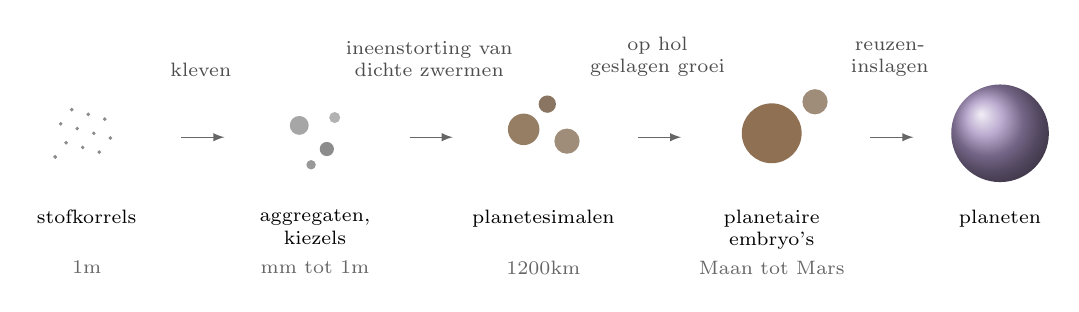
\begin{tikzpicture}[x=1cm, y=1cm, font=\scriptsize]
\foreach \x/\t/\s in {0/{stofkorrels}/{\qty{1}{\micro m}},
  2.9/{aggregaten,\\kiezels}/{mm tot \qty{1}{m}},
  5.8/{planetesimalen}/{\qtyrange{1}{200}{km}},
  8.7/{planetaire\\embryo's}/{Maan tot Mars},
  11.6/{planeten}/{} } {
  \node[align=center, anchor=north] at (\x,-0.9) {\t};
  \node[align=center, anchor=north, black!60] at (\x,-1.55) {\s};
}
\foreach \i in {0,...,11} {\fill[black!45] ({-0.4+0.07*mod(\i*7,11)},{-0.35+0.06*mod(\i*5,11)}) circle (0.025);}
\fill[black!35] (2.7,0.05) circle (0.12); \fill[black!45] (3.05,-0.25) circle (0.09);
\fill[black!40] (2.85,-0.45) circle (0.06); \fill[black!30] (3.15,0.15) circle (0.07);
\fill[brown!55!black!70] (5.55,0) circle (0.2); \fill[brown!50!black!60] (6.1,-0.15) circle (0.16);
\fill[brown!45!black!70] (5.85,0.32) circle (0.11);
\fill[brown!60!black!80] (8.7,-0.05) circle (0.38); \fill[brown!50!black!60] (9.25,0.35) circle (0.16);
\shade[ball color=blue!45!brown!60] (11.6,-0.05) circle (0.62);
\foreach \x in {1.2,4.1,7.0,9.95} {\draw[-latex, black!60] (\x,-0.1) -- +(0.55,0);}
\node[align=center, anchor=south, black!70] at (1.45,0.55) {kleven};
\node[align=center, anchor=south, black!70] at (4.35,0.55) {ineenstorting van\\dichte zwermen};
\node[align=center, anchor=south, black!70] at (7.25,0.55) {op hol\\geslagen groei};
\node[align=center, anchor=south, black!70] at (10.2,0.55) {reuzen-\\inslagen};
\end{tikzpicture}

\par\smallskip{\small Van stof tot planeten in het gebied van de rotsachtige planeten
(schematisch, niet op schaal). Korrels kleven samen tot aggregaten; zwermen kiezels storten ineen
tot \omterm{def:b2:planet-formation-meteorites:planetesimal}{planetesimalen}; de zwaartekracht laat sommige \omterm{def:b2:planet-formation-meteorites:planetesimal}{planetesimalen} op hol slaan en tot embryo's uitgroeien, die
uiteindelijk tot planeten versmelten. Voorbij de \omterm{def:b2:planet-formation-meteorites:snow-line}{sneeuwlijn} groeiden de embryo's groter en konden ze
gas vangen. Afmetingen naar Chiang en Youdin (2010) en Lugaro en anderen (2018).}
% ledger: cy10:growth, lugaro:cai
\end{omfigure}

De planeten bewaarden weinig herinnering aan deze geschiedenis: ze smolten, mengden en
herwerkten hun materie. Het archief zit in de lichamen die ophielden met groeien, de
planetoïden, en in de stukken ervan die de aarde bereiken.

\section{Meteorieten}

\begin{definition}[Meteoriet, meteorietval, meteorietvondst]
\label{def:b2:planet-formation-meteorites:fall-find}
Een \emph{meteoriet}\index{meteoriet} is een natuurlijk vast voorwerp uit de ruimte dat
zijn tocht door de dampkring heeft overleefd en de grond heeft bereikt. Een
\emph{meteorietval}\index{meteorietval} is een meteoriet die is verzameld nadat zijn
aankomst werd waargenomen, meestal als vuurbol; een
\emph{meteorietvondst}\index{meteorietvondst} is een meteoriet die op de grond is herkend zonder dat zijn val
werd gezien.
\end{definition}

De aarde veegt veel meer stof op dan stenen. Gemeten in de sneeuw van het
Antarctische plateau bereikt elk jaar ongeveer \qty{5200}{t} buitenaards stof de
grond als micrometeorieten en gesmolten bolletjes, van de zowat
\qty{15000}{t} die de dampkring binnenkomt, het meeste afgestoten door kometen en ongeveer een
vijfde door planetoïden. \omterm{def:b2:planet-formation-meteorites:fall-find}{Meteorieten}, de stenen en ijzers die groot genoeg zijn om
een voor een te worden herkend, zijn minder talrijk: de wereldcatalogus bevat er ongeveer
\num{45000}, waarvan slechts \num{1107} vallen.
% ledger: rojas21:flux, data:b4-meteorites

Het onderscheid doet ertoe. Een val wordt binnen enkele dagen verzameld, voordat regen en
zuurstof hem hebben veranderd, en elke soort \omterm{def:b2:planet-formation-meteorites:fall-find}{meteoriet} die valt, wordt even goed
verzameld; een vondst kan duizenden jaren op de grond hebben gelegen, en zijn
kans om gevonden te worden hangt af van hoe hij eruitziet en waar hij viel. De helft van alle
vondsten is in Antarctica gedaan (kader hieronder), waar systematisch wordt
gezocht. De vallen zijn de eerlijkste steekproef van wat er aankomt (figuur hieronder):
meer dan vier op de vijf zijn \omterm{def:b2:planet-formation-meteorites:chondrule}{chondrieten}, drie op de vier gewone \omterm{def:b2:planet-formation-meteorites:chondrule}{chondrieten}.
% ledger: data:b4-meteorites

\begin{omfigure}
\begin{tikzpicture}
\begin{axis}[width=0.86\linewidth, height=6.3cm, ybar, bar width=7pt,
  xmin=0.4, xmax=9.6, ymin=0.1, ymax=200, ymode=log, log origin=infty,
  xtick={1,...,9}, xticklabels={gewone, koolstofhoudende, enstatiet-, andere chondrieten,
    HED, andere achondrieten, ijzer, steenijzer, niet geclassificeerd},
  x tick label style={font=\scriptsize, rotate=30, anchor=north east, inner sep=1pt},
  tick label style={font=\scriptsize}, label style={font=\small},
  ylabel={aandeel in de steekproef (\%)}, legend pos=north east, xtick pos=bottom,
  legend style={font=\scriptsize, draw=black!30}, ymajorgrids, grid style={black!12}]
\addplot[fill=orange!70, draw=none] table[x=idx, y=falls_pct] {figdata/out/bachelor-2-meteorites-frac.dat};
\addlegendentry{vallen (\num{1107})}
\addplot[fill=blue!45, draw=none] table[x=idx, y=finds_pct] {figdata/out/bachelor-2-meteorites-frac.dat};
\addlegendentry{vondsten (\num{44534})}
\end{axis}
\end{tikzpicture}

\par\smallskip{\small \omterm{def:b2:planet-formation-meteorites:fall-find}{Meteorieten} per klasse, als percentage van de vallen en van de
vondsten (logaritmische schaal); HED: howardieten, eucrieten en diogenieten. Gegevens: NASA-export
van de Meteoritical Bulletin Database van The Meteoritical Society
(\num{45641} geldige \omterm{def:b2:planet-formation-meteorites:fall-find}{meteorieten}).}
% ledger: data:b4-meteorites
\end{omfigure}

\begin{inthefield}[Meteorieten zoeken op het blauwe ijs]
\begin{minipage}[t]{0.6\linewidth}\vspace{0pt}
Het grootste deel van de Antarctische ijskap is witte sneeuw, maar op ongeveer
\qty{1}{\percent} van haar oppervlak, waar bergen de stroming van het ijs blokkeren,
gaat elk jaar zo'n \qty{5}{cm} ijs verloren en komt kaal blauw ijs bloot. \omterm{def:b2:planet-formation-meteorites:fall-find}{Meteorieten}
die stroomopwaarts op de sneeuw vielen, over tienduizenden jaren, worden begraven,
met het ijs meegevoerd en weer aan het oppervlak gebracht waar het ijs wegslinkt:
het blauwe ijs is een val. Sinds het systematische verzamelen halverwege de jaren 1970 begon,
hebben teams op zulke velden meer dan \num{30000} exemplaren geborgen, en in
de catalogus komt de helft van alle vondsten van ten zuiden van \ang{60}~ZB. De zoekers
doorkruisen het ijs in rijen, te voet of op sneeuwscooters, en elke gevonden steen wordt
verzameld, hoe gewoon hij er ook uitziet, zodat de collectie niet scheef trekt
naar de opvallende. Elke vondst wordt gefotografeerd waar hij ligt, om
zijn context vast te leggen, en krijgt een veldnummer; later krijgt hij zijn officiële naam, een
code van drie letters voor het ijsveld, gevolgd door het jaar van het seizoen en een
volgnummer. In het curatielaboratorium worden de stenen afgeslagen met
roestvrijstalen gereedschap of droog gezaagd met een lintzaag; \omterm{def:b2:planet-formation-meteorites:chondrule}{koolstofhoudende chondrieten},
die organische verbindingen kunnen bevatten, hebben sinds 1978 een eigen kast.
\end{minipage}\hfill
\begin{minipage}[t]{0.37\linewidth}\vspace{0pt}
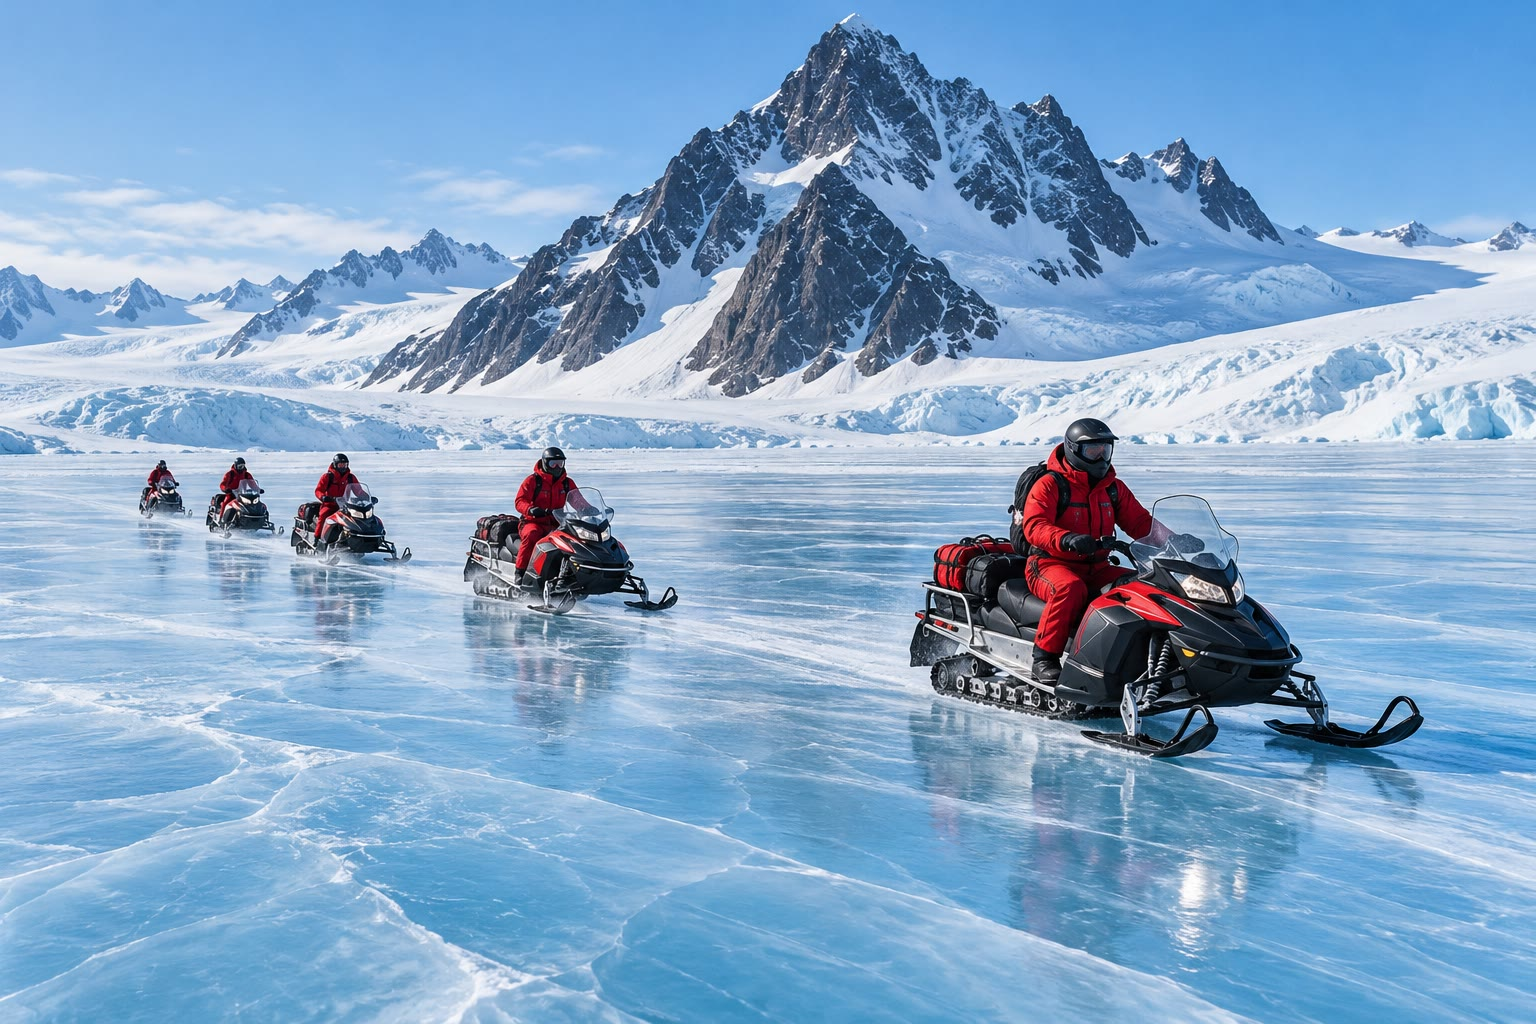
\includegraphics[width=\linewidth]{images/book4/ai/b2-blue-ice-search.jpg}

{\scriptsize Een rij zoekers op sneeuwscooters die een veld van blauw ijs doorkruist onder
een rotsige top (door AI gegenereerde illustratie).}
\end{minipage}
% ledger: folco06:blue-ice, data:b4-meteorites, nasa:antmet
\end{inthefield}

\subsection{Chondrieten}

\begin{definition}[Chondriet, koolstofhoudende chondriet, chondrule, CAI]
\label{def:b2:planet-formation-meteorites:chondrule}
Een \emph{chondriet}\index{chondriet} is een steenmeteoriet die na zijn
samenvoeging nooit is gesmolten, en waarvan de samenstelling, op de meest vluchtige
elementen na, dicht bij die van de Zon ligt. Hij bestaat grotendeels uit
\emph{chondrulen}\index{chondrule}, afgeronde druppels, van een tiende millimeter tot
ongeveer een centimeter groot, van silicaatgesteente dat uit een smelt is gestold, ingebed in
een fijnkorrelige matrix met korrels ijzer-nikkelmetaal en ijzersulfide. Sommige
chondrieten bevatten \emph{calcium-aluminiumrijke insluitsels}\index{calcium-aluminiumrijk insluitsel} (CAI's), onregelmatige witte korrels van de mineralen van calcium, aluminium
en titaan die de eerste condensaten van de nevel zijn. Een
\emph{koolstofhoudende chondriet}\index{koolstofhoudende chondriet} is een chondriet die rijk is
aan koolstof, waterhoudende mineralen en matrix, en waarvan het gehalte aan vluchtige
elementen het dichtst bij dat van de Zon komt.
\end{definition}

De \omterm{def:b2:planet-formation-meteorites:chondrule}{chondrulen} waren slechts enkele minuten gesmolten en koelden af in uren tot
dagen: een korte, plaatselijke flitsverhitting in de nevel, waarvan de oorzaak nog
onbekend is, smolt klonten stof, die als druppels stolden voordat ze
samen met stof en metaal tot een \omterm{def:b2:planet-formation-meteorites:planetesimal}{planetesimaal} werden samengeveegd. Ze vullen tot \qty{90}{\percent} van het volume van de meest
primitieve \omterm{def:b2:planet-formation-meteorites:fall-find}{meteorieten}. De CAI's maken van minder dan \qty{1}{\percent} van
gewone \omterm{def:b2:planet-formation-meteorites:chondrule}{chondrieten} tot meer dan \qty{10}{\percent} van sommige koolstofhoudende uit, en ze
ontstonden binnen ongeveer honderdduizend jaar na elkaar.
% ledger: gail:meteorites, cy10:growth, cy10:chondrules, gail:chondrite-table, lugaro:cai

\begin{omfigure}
\begin{minipage}[c]{0.5\linewidth}
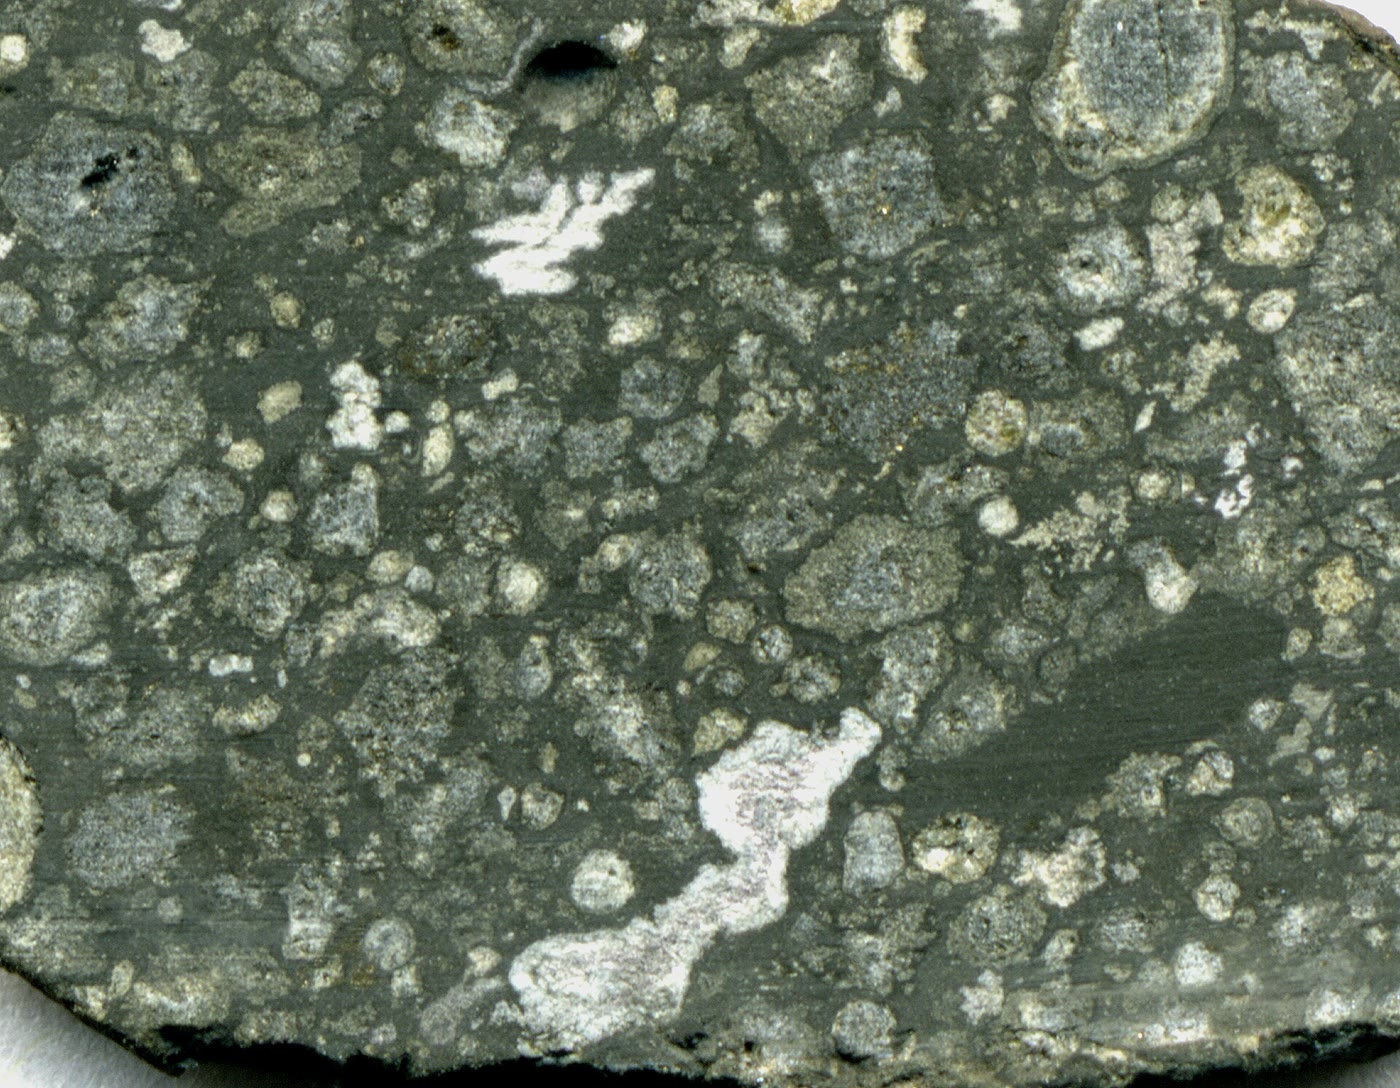
\includegraphics[width=\linewidth]{images/book4/b2-allende-chondrite.jpg}
\end{minipage}\hfill
\begin{minipage}[c]{0.46\linewidth}
{\small Een zaagvlak van de \omterm{def:b2:planet-formation-meteorites:chondrule}{koolstofhoudende chondriet} Allende (klasse CV3), die in
1969 in het noorden van Mexico viel: er werd ongeveer twee ton verzameld. De ronde grijze korrels zijn
\omterm{def:b2:planet-formation-meteorites:chondrule}{chondrulen}; de onregelmatige witte vlekken zijn CAI's; het donkere cement is de matrix. Het
beeld is enkele centimeters breed. James St.\ John, CC BY 2.0.}
\end{minipage}
% ledger: data:b4-meteorites, gail:chondrite-table
\end{omfigure}

\omterm{def:b2:planet-formation-meteorites:chondrule}{Chondrieten} vallen uiteen in groepen die verschillen in de grootte en de overvloed van hun
\omterm{def:b2:planet-formation-meteorites:chondrule}{chondrulen}, hun gehalte aan metaal, het ijzergehalte van hun olivijn en het
aandeel van hun matrix (tabel hieronder). De gewone \omterm{def:b2:planet-formation-meteorites:chondrule}{chondrieten} H, L en LL
hebben een hoog, laag en zeer laag gehalte aan metaal en aan totaal ijzer (atomaire verhoudingen
Fe/Si van \num{0.80}, \num{0.59} en \num{0.53}).
% ledger: gail:chondrite-table

\begin{table}[h]
\centering
\small
\begin{tabular}{lcccccc}
\hline
 & H & L & LL & CI & CM & CV\\
\hline
\omterm{def:b2:planet-formation-meteorites:chondrule}{chondrulen} (vol.\ \%) & 60--80 & 60--80 & 60--80 & $\ll 1$ & 20 & 45\\
gemiddelde diameter van \omterm{def:b2:planet-formation-meteorites:chondrule}{chondrulen} (mm) & 0.3 & 0.7 & 0.9 & --- & 0.3 & 1.0\\
CAI's (vol.\ \%) & 0.1--1 & 0.1--1 & 0.1--1 & $\ll 1$ & 5 & 10\\
matrix (vol.\ \%) & 10--15 & 10--15 & 10--15 & $> 99$ & 70 & 40\\
ijzer-nikkelmetaal (vol.\ \%) & 10 & 5 & 2 & 0 & 0.1 & 0--5\\
fayaliet in olivijn (mol \%) & 16--20 & 23--26 & 27--32 & & & \\
\omterm{def:b2:planet-formation-meteorites:type}{petrologische types} & 3--6 & 3--6 & 3--6 & 1 & 2 & 3\\
hoogste temperatuur (K) & 1220 & 1220 & 1220 & 430 & 670 & 870\\
\hline
\end{tabular}
\caption{Eigenschappen van de gewone (H, L, LL) en van drie groepen \omterm{def:b2:planet-formation-meteorites:chondrule}{koolstofhoudende
chondrieten}. Fayaliet: het ijzereindlid van olivijn. Gegevens: Gail en anderen (2014).}
\label{tab:b2:planet-formation-meteorites:chondrites}
% ledger: gail:chondrite-table
\end{table}

\begin{definition}[Petrologisch type]\label{def:b2:planet-formation-meteorites:type}
Het \emph{petrologisch type}\index{petrologisch type} van een \omterm{def:b2:planet-formation-meteorites:chondrule}{chondriet} is een getal
van 1 tot 6 dat vastlegt wat hem in zijn moederlichaam is overkomen: type 3 is het
minst veranderd; de types 4 tot 6 zijn steeds sterker verhit, met vervaagde \omterm{def:b2:planet-formation-meteorites:chondrule}{chondrulen}
en gerekristalliseerde mineralen van uniforme samenstelling; de types 2 en 1 zijn
steeds sterker veranderd door vloeibaar water, dat hun mineralen in klei omzette.
\end{definition}

De laatste rij van de tabel geeft de hoogste temperaturen die elke groep bereikte:
tot ongeveer \qty{1220}{K} voor de sterkst verhitte gewone \omterm{def:b2:planet-formation-meteorites:chondrule}{chondrieten}, nooit meer
dan \qty{430}{K} voor de \omterm{def:b2:planet-formation-meteorites:chondrule}{CI-chondrieten}, doordrenkt met water maar nooit heet. De
verhitting kwam, zoals de laatste paragraaf laat zien, van binnen uit de moederlichamen.
% ledger: gail:chondrite-table

\subsection{Achondrieten en ijzermeteorieten}

\begin{definition}[Achondriet, ijzermeteoriet, steenijzermeteoriet]
\label{def:b2:planet-formation-meteorites:classes}
Een \emph{achondriet}\index{achondriet} is een steenmeteoriet die is gekristalliseerd
uit een smelt of bij hoge temperatuur is gerekristalliseerd in een lichaam dat smolt, en
die dus geen \omterm{def:b2:planet-formation-meteorites:chondrule}{chondrulen} heeft. Een \emph{ijzermeteoriet}\index{ijzermeteoriet} bestaat
grotendeels uit ijzer-nikkelmetaal. Een
\emph{steenijzermeteoriet}\index{steenijzermeteoriet} bestaat uit metaal en silicaat in ongeveer
gelijke hoeveelheden.
\end{definition}

Dit zijn de stukken van lichamen die smolten en zich scheidden: \omterm{def:b2:planet-formation-meteorites:classes}{achondrieten} zijn hun
korsten en mantels, \omterm{def:b2:planet-formation-meteorites:classes}{ijzermeteorieten} hun metalen kernen, en \omterm{def:b2:planet-formation-meteorites:classes}{steenijzermeteorieten} komen van waar
metaal en silicaat elkaar raakten. De grootste familie van \omterm{def:b2:planet-formation-meteorites:classes}{achondrieten}, de howardieten,
eucrieten en diogenieten (HED), basalten en pyroxeenrijke gesteenten, maakt
\qty{5.5}{\percent} van alle vallen uit. Haar bron werd via haar spectrum en
haar baan herleid tot de planetoïde Vesta, ongeveer \qty{525}{km} groot, en de
ruimtesonde Dawn, die Vesta in 2011 bereikte, bevestigde het: de chemie
en de mineralogie van het oppervlak van Vesta komen overeen met de \omterm{def:b2:planet-formation-meteorites:fall-find}{HED-meteorieten}, een bekken
van \qty{500}{km} breed nabij de zuidpool toont waar de brokstukken werden
losgeslagen, en het zwaartekrachtsveld wijst op een ijzeren kern van ongeveer \qty{225}{km}.
Vesta smolt vroeg in haar geschiedenis bijna of helemaal. Andere \omterm{def:b2:planet-formation-meteorites:classes}{achondrieten} komen
van de Maan en van Mars. De \omterm{def:b2:planet-formation-meteorites:fall-find}{meteorieten} in de collecties lijken afkomstig
van ongeveer honderd verschillende moederlichamen.
% ledger: data:b4-meteorites, nasa:vesta-dawn, gail:meteorites

IJzermeteorieten bewaren het archief van de afkoeling van hun kernen. Een gezaagd en
met zuur geëtst vlak toont een kriskras van platen (figuur hieronder): bij hoge
temperatuur is het metaal één enkele legering van ijzer en nikkel; bij trage afkoeling groeit een
nikkelarme legering in platen langs de vlakken van het oorspronkelijke kristal,
en hoe trager de afkoeling, hoe breder de platen. Gemeten aan veel \omterm{def:b2:planet-formation-meteorites:classes}{ijzermeteorieten} geven de
plaatbreedten de afkoelingssnelheden van de kernen waaruit ze komen.
% ledger: gail:meteorites

\begin{omfigure}
\begin{minipage}[c]{0.5\linewidth}
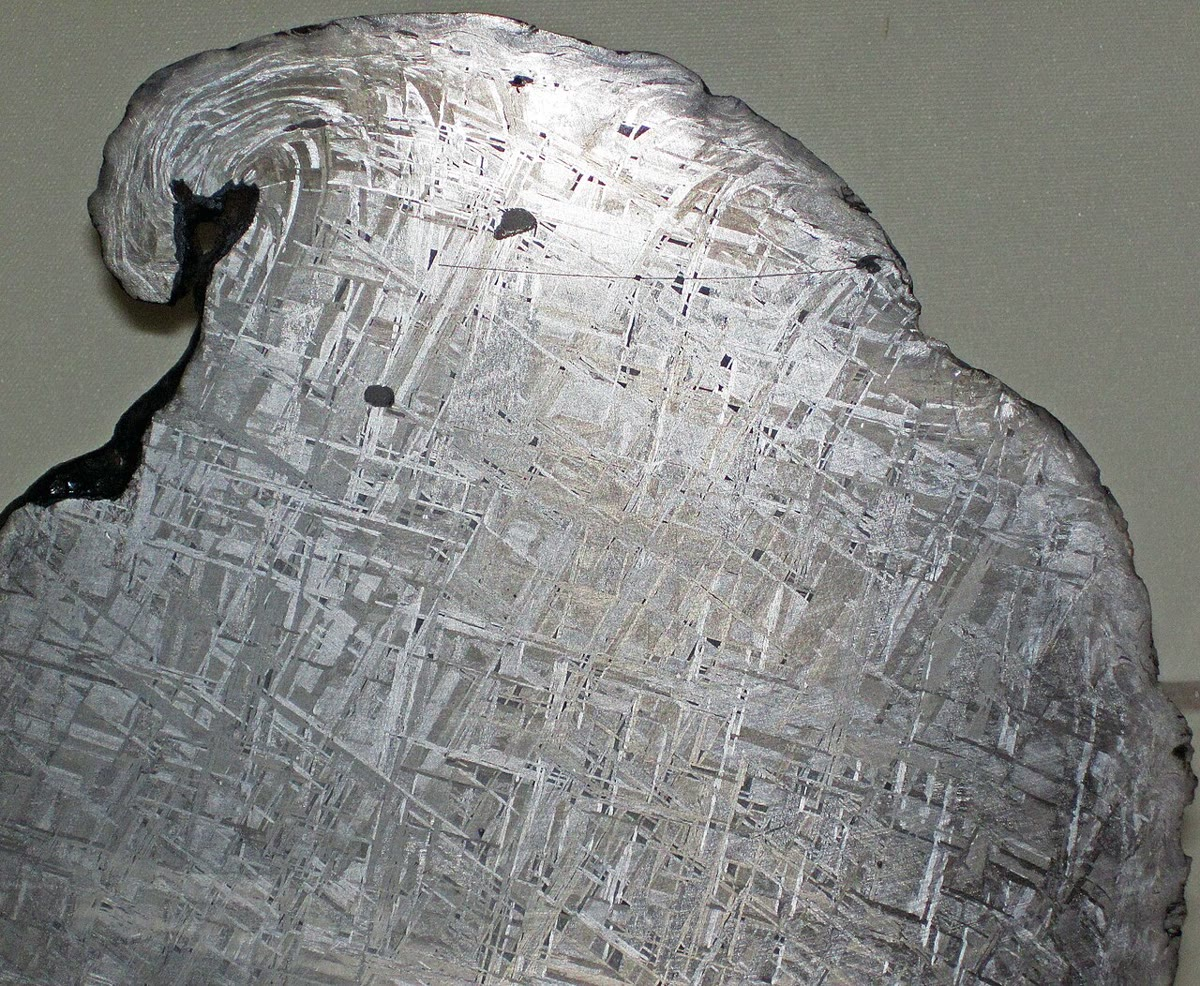
\includegraphics[width=\linewidth]{images/book4/b2-gibeon-widmanstatten.jpg}
\end{minipage}\hfill
\begin{minipage}[c]{0.46\linewidth}
{\small Het gezaagde, gepolijste en met zuur geëtste vlak van een stuk van de \omterm{def:b2:planet-formation-meteorites:classes}{ijzermeteoriet} Gibeon,
gevonden in Namibië: het kriskras van platen van ijzer-nikkellegering (het
Widmanstättenpatroon) groeide terwijl de metalen kern van zijn moederlichaam langzaam afkoelde. James St.\ John,
CC BY 2.0.}
\end{minipage}
% ledger: data:b4-meteorites
\end{omfigure}

\section{Het zonnestelsel dateren}

De ouderdom van het zonnestelsel is de ouderdom van zijn oudste vaste stoffen.
Uranium-loodisochronen van CAI's, opgesteld zoals in Boek~3, geven \qtyrange{4567}{4568}{\Ma};
de CAI's ontstonden binnen ongeveer \qty{0.1}{Myr} na elkaar, een tijd die kort
genoeg is om hun ouderdom als de geboorte van de Zon te nemen. De gebeurtenissen van de
volgende paar miljoen jaar, de vorming van \omterm{def:b2:planet-formation-meteorites:chondrule}{chondrulen} en de samenvoeging en het
smelten van de eerste lichamen, worden het best ten opzichte van de CAI's gedateerd, met klokken
die snel liepen en vroeg stilvielen.
% ledger: lugaro:cai

\begin{definition}[Kortlevend radionuclide]
\label{def:b2:planet-formation-meteorites:slr}
Een \emph{kortlevend radionuclide}\index{kortlevend radionuclide} is een
radioactief nuclide met een halveringstijd van ruwweg \num{0.1} tot \qty{100}{Myr},
dat aanwezig was toen het zonnestelsel ontstond en nu uitgestorven is, en waarvan de vroegere aanwezigheid
blijkt uit een overmaat van zijn dochter in mineralen die rijk waren aan zijn
element.
\end{definition}

Het bekendste is aluminium-26, dat vervalt tot magnesium-26 met een halveringstijd van
\qty{0.717}{Myr} (een gemiddelde levensduur van \qty{1.035}{Myr}). Toen de CAI's ontstonden, was ongeveer
één op de \num{19000} aluminiumatomen aluminium-26: de verhouding
$\ce{^{26}Al}/\ce{^{27}Al}$ was $(5.23 \pm 0.13)\times10^{-5}$, de
\emph{canonieke} waarde. Andere kortlevende nucliden bestrijken langere tijdspannes (tabel
hieronder).
% ledger: lugaro:al26, lugaro:slr-table

\begin{table}[h]
\centering
\small
\begin{tabular}{lllcc}
\hline
nuclide & dochter & referentie & halveringstijd (Myr) & beginverhouding\\
\hline
\ce{^{26}Al} & \ce{^{26}Mg} & \ce{^{27}Al} & 0.717 & $5.23\times10^{-5}$\\
\ce{^{60}Fe} & \ce{^{60}Ni} & \ce{^{56}Fe} & 2.62 & $1.0\times10^{-8}$\\
\ce{^{53}Mn} & \ce{^{53}Cr} & \ce{^{55}Mn} & 3.74 & $7\times10^{-6}$\\
\ce{^{107}Pd} & \ce{^{107}Ag} & \ce{^{108}Pd} & 6.5 & $6.6\times10^{-5}$\\
\ce{^{182}Hf} & \ce{^{182}W} & \ce{^{180}Hf} & 8.90 & $1.02\times10^{-4}$\\
\ce{^{129}I} & \ce{^{129}Xe} & \ce{^{127}I} & 15.7 & $1.28\times10^{-4}$\\
\hline
\end{tabular}
\caption{Enkele \omterm{def:b2:planet-formation-meteorites:slr}{kortlevende radionucliden} van het vroege zonnestelsel, hun stabiele
dochter, de stabiele isotoop van hetzelfde element die als referentie dient, hun
halveringstijd en hun verhouding tot de referentie toen de CAI's ontstonden. Gegevens: Lugaro en
anderen (2018).}
\label{tab:b2:planet-formation-meteorites:slr}
% ledger: lugaro:al26, lugaro:slr-table
\end{table}

\begin{proposition}[Relatieve ouderdom uit een uitgestorven nuclide]
\label{prop:b2:planet-formation-meteorites:relative-age}
Als de verhouding van een kortlevend nuclide tot zijn referentie-isotoop $R_0$ was,
overal, toen de CAI's ontstonden, en als ze in een object bij zijn vorming $R$ blijkt te zijn
geweest, dan ontstond het object
\[
  \Delta t = \tau \ln\frac{R_0}{R}
\]
na de CAI's, waarbij $\tau$ de gemiddelde levensduur van het nuclide is. Een fout
$\delta R$ op $R$ geeft de fout $\tau\,\delta R/R$ op $\Delta t$.
\end{proposition}

\begin{proof}
De referentie-isotoop is stabiel, dus de verhouding vervalt zoals het radioactieve
nuclide zelf: $R = R_0 e^{-\Delta t/\tau}$. Logaritmen nemen geeft
$\Delta t = \tau\ln(R_0/R)$. Differentiëren geeft $\mathrm d(\Delta t) =
-\tau\,\mathrm dR/R$.
\end{proof}

Een relatieve fout van \qty{10}{\percent} op de verhouding kost dus
\qty{0.1}{Myr} met aluminium-26, maar \qty{0.54}{Myr} met mangaan-53 en
\qty{1.3}{Myr} met hafnium-182: elke klok is slechts precies over enkele van zijn
eigen gemiddelde levensduren, en de juiste klok hangt af van de gebeurtenis. De verhouding $R$ in een
object wordt afgelezen uit zijn mineralen.
% ledger: lugaro:al26, lugaro:slr-table

\begin{proposition}[Aluminium-magnesiumisochroon]
\label{prop:b2:planet-formation-meteorites:al-mg}
Laat meerdere mineralen van één object samen ontstaan op het tijdstip $\Delta t$ met
dezelfde isotopische samenstelling van magnesium, $(\ce{^{26}Mg}/\ce{^{24}Mg})_0$, maar
verschillende verhoudingen $\ce{^{27}Al}/\ce{^{24}Mg}$, en sindsdien gesloten blijven. Vandaag
liggen ze op de rechte
\[
  \frac{\ce{^{26}Mg}}{\ce{^{24}Mg}}
  = \left(\frac{\ce{^{26}Mg}}{\ce{^{24}Mg}}\right)_0
  + R\,\frac{\ce{^{27}Al}}{\ce{^{24}Mg}},
\]
waarvan de helling de verhouding $R = \ce{^{26}Al}/\ce{^{27}Al}$ van het object bij zijn
vorming is.
\end{proposition}

\begin{proof}
Elk atoom aluminium-26 dat bij de vorming aanwezig was, is sindsdien een
atoom magnesium-26 geworden, dus een mineraal heeft
$\ce{^{26}Al}_{\text{toen}} = R\,\ce{^{27}Al}$ atomen magnesium-26 gewonnen, omdat aluminium-27
stabiel is. Delen door het aantal atomen magnesium-24, dat onveranderd is,
geeft de rechte.
\end{proof}

Aluminiumrijke, magnesiumarme mineralen zoals plagioklaas vertonen grote overmaten
aan magnesium-26; olivijn, vrijwel zonder aluminium, vertoont er geen. Zo werd de
tijdsvolgorde van het vroege zonnestelsel opgebouwd: eerst de CAI's; \omterm{def:b2:planet-formation-meteorites:chondrule}{chondrulen} over
de volgende paar miljoen jaar, waarbij de gegevens van de \omterm{def:b2:planet-formation-meteorites:chondrule}{chondrulen} de
levensduur van de gasschijf op minder dan vijf miljoen jaar stellen; de moederlichamen van
de \omterm{def:b2:planet-formation-meteorites:chondrule}{chondrieten} werden samengevoegd na hun jongste \omterm{def:b2:planet-formation-meteorites:chondrule}{chondrulen}. De diogenieten,
gesteenten van de mantel van Vesta, begonnen te kristalliseren binnen ongeveer een miljoen jaar na
de CAI's, en de kern van Vesta vormde zich binnen de eerste een tot
vier miljoen jaar: \omterm{def:b2:planet-formation-meteorites:classes}{ijzermeteorieten} en \omterm{def:b2:planet-formation-meteorites:classes}{achondrieten} zijn ouder dan veel
\omterm{def:b2:planet-formation-meteorites:chondrule}{chondrieten}.
% ledger: lugaro:cai, gail:vesta, gail:meteorites

\section{Warmte uit aluminium-26 en het eerste smelten}

Waar kwam de warmte vandaan die Vesta deed smelten en de gewone
\omterm{def:b2:planet-formation-meteorites:chondrule}{chondrieten} metamorfoseerde? Modellen en \omterm{def:b2:planet-formation-meteorites:fall-find}{meteorieten} zijn het erover eens dat in de vroegste lichamen
het verval van aluminium-26 de belangrijkste bron was. In gesteente van chondritische samenstelling droeg het aanvankelijk
\qty{5}{MJ} per kilogram dat binnen enkele miljoenen jaren kon vrijkomen:
genoeg om het gesteente duizenden kelvin op te warmen, als de warmte niet kon ontsnappen.
% ledger: lugaro:heat, lugaro:melting

\begin{proposition}[Opwarming van een planetesimaal door aluminium-26]
\label{prop:b2:planet-formation-meteorites:heating}
Gesteente dat per kilogram het radioactieve vermogen $H_0 e^{-t/\tau}$ ontvangt,
de soortelijke warmte $c$ heeft en geen warmte verliest, warmt na zijn accretie op
het tijdstip $t_a$ op als
\[
  T(t) = T_0 + \frac{H_0\tau}{c}\left(e^{-t_a/\tau} - e^{-t/\tau}\right),
\]
en nadert de piektemperatuur
$T_{\max} = T_0 + (H_0\tau/c)\,e^{-t_a/\tau}$. Een kritische temperatuur
$T_c > T_0$ wordt alleen bereikt als het lichaam is samengevoegd vóór
\[
  t_a^* = \tau\ln\frac{H_0\tau}{c\,(T_c - T_0)}.
\]
\end{proposition}

\begin{proof}
Zonder verliezen is $c\,\mathrm dT/\mathrm dt = H_0 e^{-t/\tau}$. Integreren vanaf
$t_a$, waar $T = T_0$, geeft
$c\,(T - T_0) = H_0\tau\,(e^{-t_a/\tau} - e^{-t/\tau})$, wat nadert tot
$H_0\tau e^{-t_a/\tau}$ als $t \to \infty$. $T_{\max} = T_c$ stellen en oplossen
naar $t_a$ geeft $t_a^*$; bij een vroegere accretie ligt de piek hoger.
\end{proof}

Een model van het moederlichaam van de gewone \omterm{def:b2:planet-formation-meteorites:chondrule}{chondrieten} gebruikt
$H_0 = \qty{1.9e-7}{W.kg^{-1}}$, $c = \qty{837}{J.kg^{-1}.K^{-1}}$ en
$T_0 = \qty{250}{K}$. Dan is $H_0\tau/c$ ongeveer \qty{7400}{K}. Drie
temperaturen doen ertoe: rond \qty{750}{K} begint het poreuze gesteente te sinteren tot een
compact gesteente; rond \qty{1200}{K} beginnen het metaal en het ijzersulfide samen
te smelten; rond \qty{1700}{K} smelten de laatste silicaten. Een lichaam dat
vóór \qty{1.7}{Myr} was samengevoegd, smolt volledig; vóór \qty{2.1}{Myr} smolten zijn metaal en sulfide
en konden ze tot een kern wegzakken; tot ongeveer \qty{2.8}{Myr} werd het minstens
gesinterd en gemetamorfoseerd; latere lichamen bleven koel (figuur hieronder).
% ledger: gail:params, gail:temps, lugaro:al26

\begin{omfigure}
\begin{tikzpicture}
\begin{axis}[omrecord, name=left, width=0.45\linewidth, height=6.0cm,
  xmin=0, xmax=8, ymin=0, ymax=2300,
  xlabel={tijd na de CAI's (Myr)}, ylabel={temperatuur (K)},
  tick label style={font=\scriptsize}, label style={font=\small}]
\addplot[black!45, densely dashed, domain=0:8, samples=2] {750};
\addplot[black!45, densely dashed, domain=0:8, samples=2] {1200};
\addplot[black!45, densely dashed, domain=0:8, samples=2] {1700};
\addplot[thick, red!75!black] table[x=t_Myr, y=T_K] {figdata/out/bachelor-2-al26-ta15.dat};
\addplot[thick, orange!80!black] table[x=t_Myr, y=T_K] {figdata/out/bachelor-2-al26-ta20.dat};
\addplot[thick, teal!70!black] table[x=t_Myr, y=T_K] {figdata/out/bachelor-2-al26-ta25.dat};
\addplot[thick, blue!70!black] table[x=t_Myr, y=T_K] {figdata/out/bachelor-2-al26-ta30.dat};
\node[font=\tiny, red!75!black, anchor=south east] at (axis cs:7.9,1995) {$t_a = \qty{1.5}{Myr}$};
\node[font=\tiny, orange!80!black, anchor=south east] at (axis cs:7.9,1325) {2};
\node[font=\tiny, teal!70!black, anchor=south east] at (axis cs:7.9,915) {2.5};
\node[font=\tiny, blue!70!black, anchor=north east] at (axis cs:7.9,650) {3};
\node[font=\tiny, black!60, anchor=south west] at (axis cs:0.1,1700) {silicaten gesmolten};
\node[font=\tiny, black!60, anchor=south west] at (axis cs:0.1,1200) {Fe--FeS smelt};
\node[font=\tiny, black!60, anchor=south west] at (axis cs:0.1,750) {sinteren};
\end{axis}
\begin{axis}[omrecord, at={(left.east)}, anchor=west, xshift=2.1cm, width=0.45\linewidth,
  height=6.0cm, xmin=0, xmax=4, ymin=0, ymax=8000,
  xlabel={accretietijdstip $t_a$ (Myr)}, ylabel={piektemperatuur (K)},
  tick label style={font=\scriptsize}, label style={font=\small},
  scaled y ticks=false, yticklabel style={/pgf/number format/1000 sep={\,}}]
\addplot[black!45, densely dashed, domain=0:4, samples=2] {750};
\addplot[black!45, densely dashed, domain=0:4, samples=2] {1200};
\addplot[black!45, densely dashed, domain=0:4, samples=2] {1700};
\addplot[thick, black] table[x=ta_Myr, y=Tpeak_K] {figdata/out/bachelor-2-al26-peak.dat};
\draw[black!60] (axis cs:1.69,0) -- (axis cs:1.69,1700);
\draw[black!60] (axis cs:2.13,0) -- (axis cs:2.13,1200);
\node[font=\tiny, black!70, anchor=south] at (axis cs:2.0,4500) {\qty{1.7}{Myr}};
\draw[black!50, -latex] (axis cs:2.0,4450) -- (axis cs:1.71,1800);
\node[font=\tiny, black!70, anchor=south] at (axis cs:2.9,3300) {\qty{2.1}{Myr}};
\draw[black!50, -latex] (axis cs:2.9,3250) -- (axis cs:2.16,1300);
\end{axis}
\end{tikzpicture}

\par\smallskip{\small Opwarming door aluminium-26 van het binnenste van een chondritisch lichaam zonder
warmteverlies (de propositie hierboven; $H_0 = \qty{1.9e-7}{W.kg^{-1}}$,
$c = \qty{837}{J.kg^{-1}.K^{-1}}$, $T_0 = \qty{250}{K}$, $\tau = \qty{1.035}{Myr}$).
Links: temperatuur tegen de tijd voor lichamen die 1.5, 2, 2.5 en \qty{3}{Myr}
na de CAI's zijn samengevoegd. Rechts: piektemperatuur tegen accretietijdstip; lichamen die
vóór \qty{1.7}{Myr} waren samengevoegd, smolten, vóór \qty{2.1}{Myr} smolten hun metaal en sulfide.
Werkelijke lichamen besteden een deel van de warmte aan smelten, wat de temperatuur begrenst, en verliezen
warmte nabij hun oppervlak. Modelwaarden: Gail en anderen (2014).}
% ledger: gail:params, gail:temps, lugaro:al26
\end{omfigure}

De propositie verwaarloost warmteverlies, wat alleen diep in een groot lichaam opgaat.
Warmte diffundeert over de afstand $\sqrt{\kappa t}$ in de tijd $t$, waarbij
$\kappa$ de thermische diffusiviteit van het gesteente is: met de waarden van het model
ongeveer \qty{5}{km} in één gemiddelde levensduur van aluminium-26 (\cref{exo:b2:planet-formation-meteorites:12}). Lichamen die veel
kleiner zijn, verliezen hun warmte even snel als ze die maken; gedetailleerde modellen laten zien
dat lichamen van meer dan \qtyrange{10}{20}{km} groot konden smelten.
% ledger: gail:params, lugaro:melting

\begin{definition}[Planetaire differentiatie]
\label{def:b2:planet-formation-meteorites:differentiation}
\emph{Planetaire differentiatie}\index{planetaire differentiatie} is de
scheiding van een lichaam, eenmaal gesmolten of gedeeltelijk gesmolten, in lagen van verschillende
samenstelling en dichtheid: een metalen kern, een silicaatmantel en een korst die uit
de laatste smelten bestaat.
\end{definition}

De \omterm{def:b2:planet-formation-meteorites:fall-find}{meteorieten} leggen zo twee soorten vroege lichamen vast. Die welke binnen
ongeveer de eerste twee miljoen jaar ontstonden, hadden genoeg aluminium-26 om te smelten en
te differentiëren: hun kernen zijn de \omterm{def:b2:planet-formation-meteorites:classes}{ijzermeteorieten}, hun korsten en mantels
de \omterm{def:b2:planet-formation-meteorites:classes}{achondrieten}, Vesta de overlevende. Die welke later ontstonden, bleven
\omterm{def:b2:planet-formation-meteorites:chondrule}{chondrieten}, van binnenuit verhit in een mate die bepaald werd door hun geboortedatum en door
de diepte van elk brokstuk: de diepste werden type 6, de ondiepste bleven
type 3. De aarde zelf, opgebouwd uit embryo's en \omterm{def:b2:planet-formation-meteorites:planetesimal}{planetesimalen} van beide soorten en
getroffen door reuzeninslagen, differentieerde in haar kern, mantel en korst.
% ledger: gail:meteorites, gail:vesta, gail:temps

\section{Oefeningen}

\begin{exercise}[$\star$]\label{exo:b2:planet-formation-meteorites:1}
Bereken in de \omterm{def:b2:planet-formation-meteorites:nebula}{zonnenevel} met minimale massa de oppervlaktedichtheid van het gas op
\qty{1}{au} en op \qty{5.2}{au}, en de oppervlaktedichtheid van de vaste stoffen op
\qty{1}{au} (alleen gesteente, $Z_{\mathrm{rel}} = 0.33$) en op \qty{5.2}{au} (al het ijs
gecondenseerd, $Z_{\mathrm{rel}} = 1$). Hoeveel keer zwaarder dan de vaste stoffen is het
gas op \qty{5.2}{au}?
% ledger: cy10:mmsn
\end{exercise}

\begin{exercise}[$\star$]\label{exo:b2:planet-formation-meteorites:2}
Rangschik met de figuur van de \omterm{def:b2:planet-formation-meteorites:condensation}{condensatietemperaturen} aluminium, natrium,
magnesium, ijzer, zwavel en zuurstof (als waterijs) van het eerste tot het laatste dat
condenseert, en geef de vluchtigheidsgroep van elk. Welke zou men verrijkt verwachten
in CAI's, en welke verarmd in de aarde vergeleken met de Zon?
% ledger: lodders:tc-table, lodders:groups
\end{exercise}

\begin{exercise}[$\star$]\label{exo:b2:planet-formation-meteorites:3}
De catalogus vermeldt \num{1107} vallen, waarvan 856 gewone \omterm{def:b2:planet-formation-meteorites:chondrule}{chondrieten} en
49 \omterm{def:b2:planet-formation-meteorites:classes}{ijzermeteorieten}, en \num{44534} vondsten, waarvan \num{38647} gewone \omterm{def:b2:planet-formation-meteorites:chondrule}{chondrieten},
\num{1020} \omterm{def:b2:planet-formation-meteorites:classes}{ijzermeteorieten}, en \num{22096} van ten zuiden van \ang{60}~ZB. Bereken het
aandeel gewone \omterm{def:b2:planet-formation-meteorites:chondrule}{chondrieten} en \omterm{def:b2:planet-formation-meteorites:classes}{ijzermeteorieten} onder de vallen en onder de vondsten,
en het aandeel Antarctische vondsten. Welke steekproef zou men gebruiken om de
verhoudingen te schatten waarin de klassen op de aarde aankomen, en waarom?
% ledger: data:b4-meteorites
\end{exercise}

\begin{exercise}[$\star$]\label{exo:b2:planet-formation-meteorites:4}
De mineralen van een object geven de beginverhouding
$\ce{^{26}Al}/\ce{^{27}Al} = \num{1.0e-5}$. Hoe lang na de CAI's ontstond het?
Neem $R_0 = \num{5.23e-5}$ en een gemiddelde levensduur van \qty{1.035}{Myr}.
% ledger: lugaro:al26
\end{exercise}

\begin{exercise}[$\star\star$]\label{exo:b2:planet-formation-meteorites:5}
Bereken met \cref{prop:b2:planet-formation-meteorites:disc-mass}, met
$\Sigma_1 = \qty{2.2e4}{kg.m^{-2}}$ op \qty{1}{au} (\qty{1}{au} $=
\qty{1.496e11}{m}$, $M_\odot = \qty{1.989e30}{kg}$), de massa van de
nevel met minimale massa binnen \qty{30}{au} en binnen \qty{100}{au}, in zonsmassa's.
Vergelijk met de waargenomen schijven, \numrange{0.001}{0.1} zonsmassa.
% ledger: cy10:mmsn
\end{exercise}

\begin{exercise}[$\star\star$]\label{exo:b2:planet-formation-meteorites:6}
Zoek in de passieve schijf $T = \qty{120}{K}\,(r/\qty{1}{au})^{-3/7}$ waar waterijs
(\qty{182}{K}) en methaanijs (\qty{41}{K}) stabiel worden. Een korrel in direct
zonlicht bereikt \qty{182}{K} op \qty{2.3}{au}. Waarom verschillen de twee schattingen van de
\omterm{def:b2:planet-formation-meteorites:snow-line}{sneeuwlijn}, en welke is van toepassing op de lichamen waaruit de planeten zijn opgebouwd?
% ledger: cy10:passive, lodders:phases
\end{exercise}

\begin{exercise}[$\star\star$]\label{exo:b2:planet-formation-meteorites:7}
Bereken de isolatiemassa, met $b = 5$, van een embryo op \qty{1}{au} in de
nevel met minimale massa ($\Sigma_p = \qty{10.9}{g.cm^{-2}}$), en op \qty{5.2}{au}
voorbij de \omterm{def:b2:planet-formation-meteorites:snow-line}{sneeuwlijn} ($\Sigma_p = \qty{2.78}{g.cm^{-2}}$), in aardmassa's
($M_\oplus = \qty{5.972e24}{kg}$, $M_\odot = \qty{1.989e30}{kg}$). Wat wordt ze
op \qty{5.2}{au} in een schijf met \num{3.5} keer meer vaste stoffen?
% ledger: cy10:isolation, cy10:mmsn, earth:mass
\end{exercise}

\begin{exercise}[$\star\star$]\label{exo:b2:planet-formation-meteorites:8}
Gesteente van CI-samenstelling bevatte \num{1.01e16} atomen aluminium-26 per gram toen
de CAI's ontstonden, en elk verval laat \qty{5.00e-13}{J} warmte achter. Bereken de
warmte die per kilogram over het hele verval vrijkomt, en de temperatuurstijging die ze
zou geven met $c = \qty{837}{J.kg^{-1}.K^{-1}}$ en zonder verliezen. Hoeveel keer
meer is dat dan de warmte die nodig is om het gesteente op te warmen van \num{250} tot
\qty{1700}{K}?
% ledger: lugaro:heat, gail:params
\end{exercise}

\begin{exercise}[$\star\star$]\label{exo:b2:planet-formation-meteorites:9}
Over zijn hele verval maakt aluminium-26 \qty{5.07e10}{erg} per gram CI-gesteente
vrij en ijzer-60 \qty{7.49e7}{erg} per gram. Bereken de verhouding van de twee
energieën. De halveringstijd van ijzer-60 is \qty{2.62}{Myr}: bereken zijn gemiddelde levensduur,
en de verhouding van de twee aanvankelijke verwarmingsvermogens, energie gedeeld door gemiddelde levensduur.
% ledger: lugaro:heat, lugaro:slr-table, lugaro:al26
\end{exercise}

\begin{exercise}[$\star\star\star$]\label{exo:b2:planet-formation-meteorites:10}
Zoek met de resultaten van \cref{exo:b2:planet-formation-meteorites:9} het tijdstip waarna ijzer-60 gesteente
sneller verwarmt dan aluminium-26. Had ijzer-60 een lichaam dat zo laat werd samengevoegd,
kunnen doen smelten? (Vergelijk de energie die het dan nog moet vrijmaken met de
\qty{1.2e6}{J.kg^{-1}} die nodig is om gesteente op te warmen van \num{250} tot \qty{1700}{K}.)
% ledger: lugaro:heat, lugaro:slr-table, lugaro:al26
\end{exercise}

\begin{exercise}[$\star\star\star$]\label{exo:b2:planet-formation-meteorites:11}
Bereken met $H_0 = \qty{1.9e-7}{W.kg^{-1}}$, $\tau = \qty{1.035}{Myr}$,
$c = \qty{837}{J.kg^{-1}.K^{-1}}$ en $T_0 = \qty{250}{K}$ (een jaar van
\qty{3.156e7}{s}) de laatste accretietijdstippen waarvoor het centrum van een
groot lichaam \qty{1200}{K} en \qty{1700}{K} bereikt. Sommige metingen wijzen erop dat
het aanvankelijke aluminium-26 in delen van de schijf slechts de helft van de canonieke waarde bedroeg:
hoeveel zouden beide tijdstippen verschuiven? Toon aan dat de verschuiving niet afhangt van de
kritische temperatuur.
% ledger: gail:params, gail:temps, lugaro:al26
\end{exercise}

\begin{exercise}[$\star\star\star$]\label{exo:b2:planet-formation-meteorites:12}
Gesteente met een geleidbaarheid van \qty{2.1}{W.m^{-1}.K^{-1}}, een dichtheid van
\qty{3300}{kg.m^{-3}} en een soortelijke warmte van \qty{837}{J.kg^{-1}.K^{-1}} heeft
de thermische diffusiviteit $\kappa = k/(\rho c)$. Bereken die, en de afstand
$\sqrt{\kappa\tau}$ waarover warmte diffundeert in één gemiddelde levensduur van aluminium-26.
Leg uit waarom de propositie over de opwarming van toepassing is op het centrum van een lichaam
van \qty{100}{km} groot, maar niet op een lichaam van \qty{2}{km}, en vergelijk met de
kleinste lichamen die konden smelten, van \qtyrange{10}{20}{km} groot.
% ledger: gail:params, lugaro:melting, lugaro:al26
\end{exercise}

\section{Probleem: De steen die op het bevroren meer viel}

\begin{problem}[{Weekendprobleem --- een pas gevallen steen classificeren, zijn
chondrulen dateren met aluminium-26, en bepalen hoe heet zijn moederlichaam werd}]
\label{pb:b2:planet-formation-meteorites:1}
% values: calc/ch02.py
% ledger: data:b4-meteorites, gail:chondrite-table, lugaro:al26, lugaro:cai, gail:params, gail:temps, cy10:mmsn, cy10:isolation, lodders:tc-table, earth:mass
Op een winternacht trekt een vuurbol door de hemel boven een verzonnen noordelijk meer,
en klinkt er een knal. De volgende ochtend wordt een steen met een zwarte korst van \qty{2.4}{kg}
van het ijs opgeraapt, midden in een verse krater in de sneeuw. De gezaagde
steen toont \omterm{def:b2:planet-formation-meteorites:chondrule}{chondrulen} die \qty{75}{\percent} van zijn volume uitmaken, gemiddeld \qty{0.3}{mm}
groot, met vage randen; metaal maakt \qty{9}{\percent} van zijn
volume uit, en zijn olivijn bevat 18 molprocent fayaliet. Een laboratorium
analyseert één \omterm{def:b2:planet-formation-meteorites:chondrule}{chondrule} (tabel hieronder). Gebruik de tabellen van het hoofdstuk,
$R_0 = \num{5.23e-5}$, $\tau = \qty{1.035}{Myr}$, een jaar van \qty{3.156e7}{s},
$H_0 = \qty{1.9e-7}{W.kg^{-1}}$, $c = \qty{837}{J.kg^{-1}.K^{-1}}$,
$T_0 = \qty{250}{K}$, een geleidbaarheid van \qty{2.1}{W.m^{-1}.K^{-1}}, een dichtheid van
\qty{3300}{kg.m^{-3}}, \qty{1}{au} $= \qty{1.496e11}{m}$,
$M_\odot = \qty{1.989e30}{kg}$ en $M_\oplus = \qty{5.972e24}{kg}$.

\begin{center}
\small
\begin{tabular}{lcc}
\hline
mineraal & $\ce{^{27}Al}/\ce{^{24}Mg}$ & $\ce{^{26}Mg}/\ce{^{24}Mg}$\\
\hline
olivijn & 0.05 & \num{0.139500}\\
glas & 3.00 & \num{0.139518}\\
plagioklaas & 15.0 & \num{0.139590}\\
\hline
\end{tabular}
\end{center}

\medskip
\noindent\textbf{Deel I --- De steen.}
\begin{enumerate}
  \item Is de steen een val of een vondst? Waarom maakt dat hem waardevol?
  \item Van de \num{1107} vallen van de catalogus zijn er 856 gewone \omterm{def:b2:planet-formation-meteorites:chondrule}{chondrieten}. Hoe groot
        is de kans dat een willekeurig gekozen val er een is?
  \item Zeg met de tabel van de chondrietgroepen tot welke groep de steen behoort.
  \item Zijn \omterm{def:b2:planet-formation-meteorites:chondrule}{chondrulen} hebben vage randen en zijn mineralen hebben een uniforme
        samenstelling. Op welke \omterm{def:b2:planet-formation-meteorites:type}{petrologische types} wijst dat, en wat is de
        hoogste temperatuur die zijn groep bereikte, in kelvin en in graden Celsius?
  \item Waarom zou men er weinig CAI's in verwachten, en waarom is de steen toch
        jonger dan elke CAI?
\end{enumerate}

\noindent\textbf{Deel II --- Wanneer ontstond de chondrule?}
\begin{enumerate}[resume]
  \item Leg uit waarom de verhouding $\ce{^{26}Mg}/\ce{^{24}Mg}$ van mineraal tot mineraal
        stijgt met $\ce{^{27}Al}/\ce{^{24}Mg}$.
  \item Bereken uit het olivijn en het plagioklaas de helling van de isochroon.
        Wat meet ze?
  \item Ga na dat het glas op dezelfde rechte ligt.
  \item Hoe lang na de CAI's ontstond de \omterm{def:b2:planet-formation-meteorites:chondrule}{chondrule}?
  \item Neem voor de CAI's een ouderdom van \qty{4567.5}{\Ma} en geef de ouderdom van de \omterm{def:b2:planet-formation-meteorites:chondrule}{chondrule}.
  \item Hoe groot zou de verhouding $\ce{^{26}Al}/\ce{^{27}Al}$ zijn geweest in een mineraal dat
        \qty{10}{Myr} na de CAI's ontstond? Welk nuclide van de tabel zou zo'n
        gebeurtenis beter dateren?
\end{enumerate}

\noindent\textbf{Deel III --- De opwarming van het moederlichaam.}
Het moederlichaam van de steen, met een straal van \qty{20}{km}, werd \qty{2.4}{Myr} na
de CAI's samengevoegd, kort na zijn \omterm{def:b2:planet-formation-meteorites:chondrule}{chondrulen}.
\begin{enumerate}[resume]
  \item Bereken de thermische diffusiviteit van het gesteente en de tijd $R^2/\kappa$ die
        warmte nodig heeft om uit het centrum te ontsnappen, in miljoenen jaren. Mag men het centrum
        behandelen alsof het geen warmte verliest?
  \item Bereken het verwarmingsvermogen van aluminium-26 per kilogram gesteente op het tijdstip
        van samenvoeging.
  \item Bereken de warmte die na de samenvoeging per kilogram nog moet vrijkomen.
  \item Bereken de temperatuurstijging en de piektemperatuur in het centrum.
  \item Vergelijk met de drie kritische temperaturen van het hoofdstuk. Is het
        centrum gesmolten? Strookt dit met vraag 4?
  \item Wat is het laatste tijdstip van samenvoeging waarvoor het metaal en het sulfide van het
        centrum zouden zijn beginnen te smelten?
  \item Hoe lang na de samenvoeging is \qty{90}{\percent} van de temperatuurstijging
        bereikt? Geef de datum na de CAI's.
\end{enumerate}

\noindent\textbf{Deel IV --- De buren.}
\begin{enumerate}[resume]
  \item Een \omterm{def:b2:planet-formation-meteorites:classes}{achondriet} komt van een lichaam dat \qty{0.8}{Myr} na de
        CAI's werd samengevoegd. Bereken de piektemperatuur die de propositie zou geven, en zeg
        wat er werkelijk met het lichaam gebeurde.
  \item Hoeveel keer meer aluminium-26 per kilogram had dat lichaam bij zijn
        samenvoeging dan het moederlichaam van de steen?
  \item De steen is armer dan de Zon aan zink en lood, maar niet aan magnesium of
        aluminium. Verklaar dat met de \omterm{def:b2:planet-formation-meteorites:condensation}{condensatietemperaturen}.
  \item Bereken in de nevel met minimale massa de oppervlaktedichtheid van gesteente
        ($Z_{\mathrm{rel}} = 0.33$) op \qty{2.5}{au}, waar het moederlichaam
        draaide.
  \item Bereken de isolatiemassa op \qty{2.5}{au}, met $b = 5$, in kilogram en
        in aardmassa's, en vergelijk ze met de massa van het moederlichaam.
  \item Geef de piektemperatuur van het centrum van het moederlichaam, het kerngetal
        van dit probleem, in graden Celsius.
\end{enumerate}
\end{problem}
